\documentclass[12pt]{article}
\usepackage[utf8]{inputenc}
\usepackage[T2A]{fontenc}
\usepackage[mongolian]{babel}
\usepackage{graphicx}
\title{Сургуулийн онлайн веб сайт}
\begin{document}
	\maketitle
	\section{Хэрэглэгчийн судалгаа}
	Хүмүүсийн хоорондын харилцааны томоохон хэсгийг эзлэх social орчин нь илүү олныг хамрах болсноор түүнийгээ дагаад хэрэглэгчийн шаардлагууд ч нэмэгдсэн. Facebook messenger-г хүмүүс өдөр тутамдаа харилцааны гол хэрэгсэл болгон ашиглаж байна. Интернэт орчинд чатлаж байгаа хүмүүс нүүр нүүрээ харан харилцахгүй байгаа ч гэсэн нөгөө хүнийхээ явуулсан Sticker emoji зэргээс тухайн хүн ямар хариу үйлдэл үзүүлж байгаа, ямар сэтгэгдэлтэй байгаа зэргийг Sticker зураг хараад хялбар ойлгох боломжтой болсон. Манай энэхүү систем нь ч мөн тэр шаардлагыг хангахыг зорьсон.
	\section{Ижил төстэй програм}
	\begin{itemize}
	\item Facebook
	\end{itemize}
	\begin{figure}
	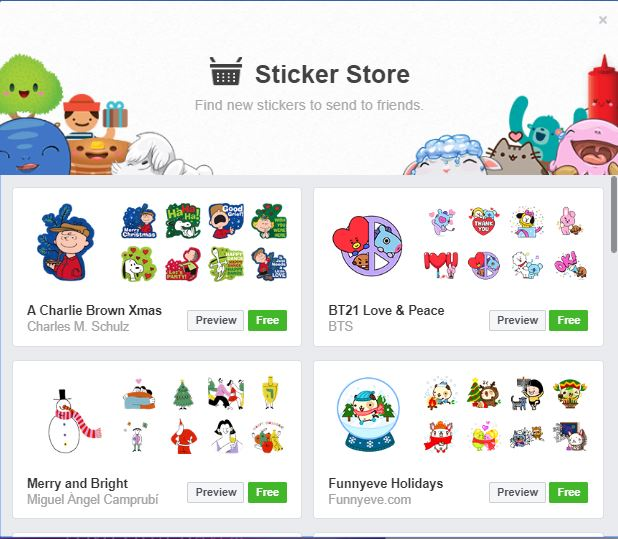
\includegraphics[width=\linewidth]{store.jpg}
	\caption{fb.}
	\label{fig:bpmn1}
	\end{figure}
	\begin{figure}
	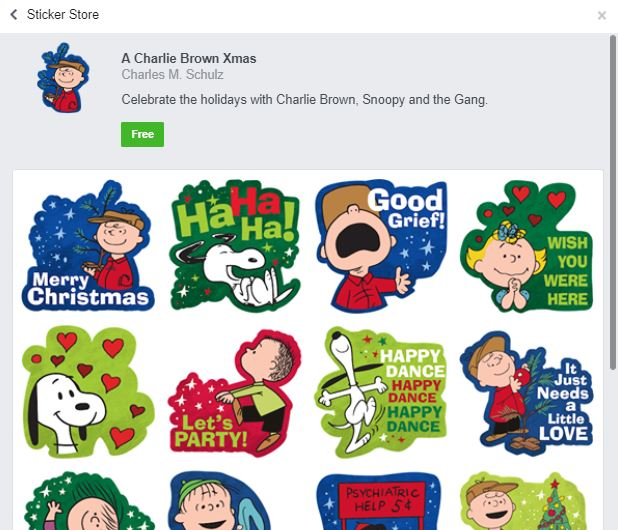
\includegraphics[width=\linewidth]{review.jpg}
	\caption{fb.}
	\label{fig:bpmn1}
\end{figure}
	\begin{figure}
		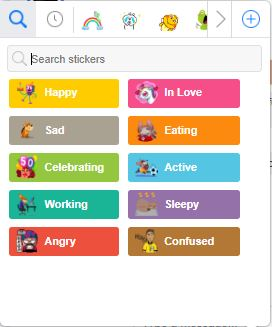
\includegraphics[width=\linewidth]{oor.jpg}
		\caption{fb.}
		\label{fig:bpmn1}
	\end{figure}
		Rasmus Lerdorf WWW-д вэб хуудас үүсгэх үедээ өгөгдөл боловсруулах хялбархан арга хайж байгаад 1995 онд PHP хэлийг скрипт хэл байдлаар зохиосон. PHP нь сервер талын скрипт хэл ба динамик вэб хуудас хийхэд илүү тохиромжтой. Энэ скрипт хэл нь энгийн хэрэглээний вэб сайтаас эхлээд байгууллагын иж бүрэн вэб программ хийж болохоор MySQL мэтийн өгөгдлийн сантай харилцан ажиллах боломжтой. Хуудас ачаалах үед броузерээр нэг бүрчлэн уншдаг HTML-тэй адилгүй, PHP баримтыг бэлтгэхдээ серверээр урьдчилан боловсруулдаг. PHP код агуулсан хуудас нь хэрэглэгчийн броузерт илгээгдхээс өмнө серверээр боловсруулагдсан байдаг. PHP хэлний өөр нэг давуу тал бол скриптэн хэл юм. Ихэнх програмчлалын хэлнүүдэд ажиллахын өмнө машины хэл рүү хөрвүүлэх тусгай файлууд /compile/ шаардлагатай байдаг бол PHP хэлний хувьд хөрвүүлэлт хийх шаардлагагүй байдаг тул код засварлах болон шалгахад илүү хурдан байдаг.
	\section{Төслийн ажлын зорилго}
	Энэхүү систем нь бусад онлайн харилцааны хэрэгслүүдтэй адил хэрэглэгчийн сэтгэл ханамжийг бий болгох зорилгоор чатын хэсэгт стикер эможи зэргийг нэмж оруулах зорилготой.
	\section{Системийн шаардлага}
	\begin{itemize}
		\item Систем нь веб суурьтай байх.
		\item Системийг ашиглахын тулд заавал сүлжээнд холбогдсон байх.
		\item Google хаягаар бүртгүүлэх боломжтой байх.
	\end{itemize}
	\section{Системийн хэрэглэгчид}
	\begin{enumerate}
		\item Багш
		\item Оюутан
		\item Сургалтын алба
		\item Системийн администратор
	\end{enumerate}
	\section{Функционал шаардлага}
		\begin{itemize}
			\item Стикер нэмэх, устгах
			\item Стикерийн жагсаалт харах
			\item Сонирхсон стикерийн дэлгэрэнгүй харах
			\item Стикер татах, илгээх
			\item Татсан стикер харах
		\end{itemize}
	\section{Функциональ бус шаардлага}	
		\begin{itemize}
			\item Системийн загвар ашиглахад хялбар ойлгомжтой байх
			\item Бүх төрлийн төхөөрөмжид тохиромжтой хэлбэрээр харагддаг /респонсив/ загвартай байна.
			\item  Юникодыг дэмждэг байх шаардлагатай хийгдэнэ.		
		\end{itemize}
		\begin{figure}
			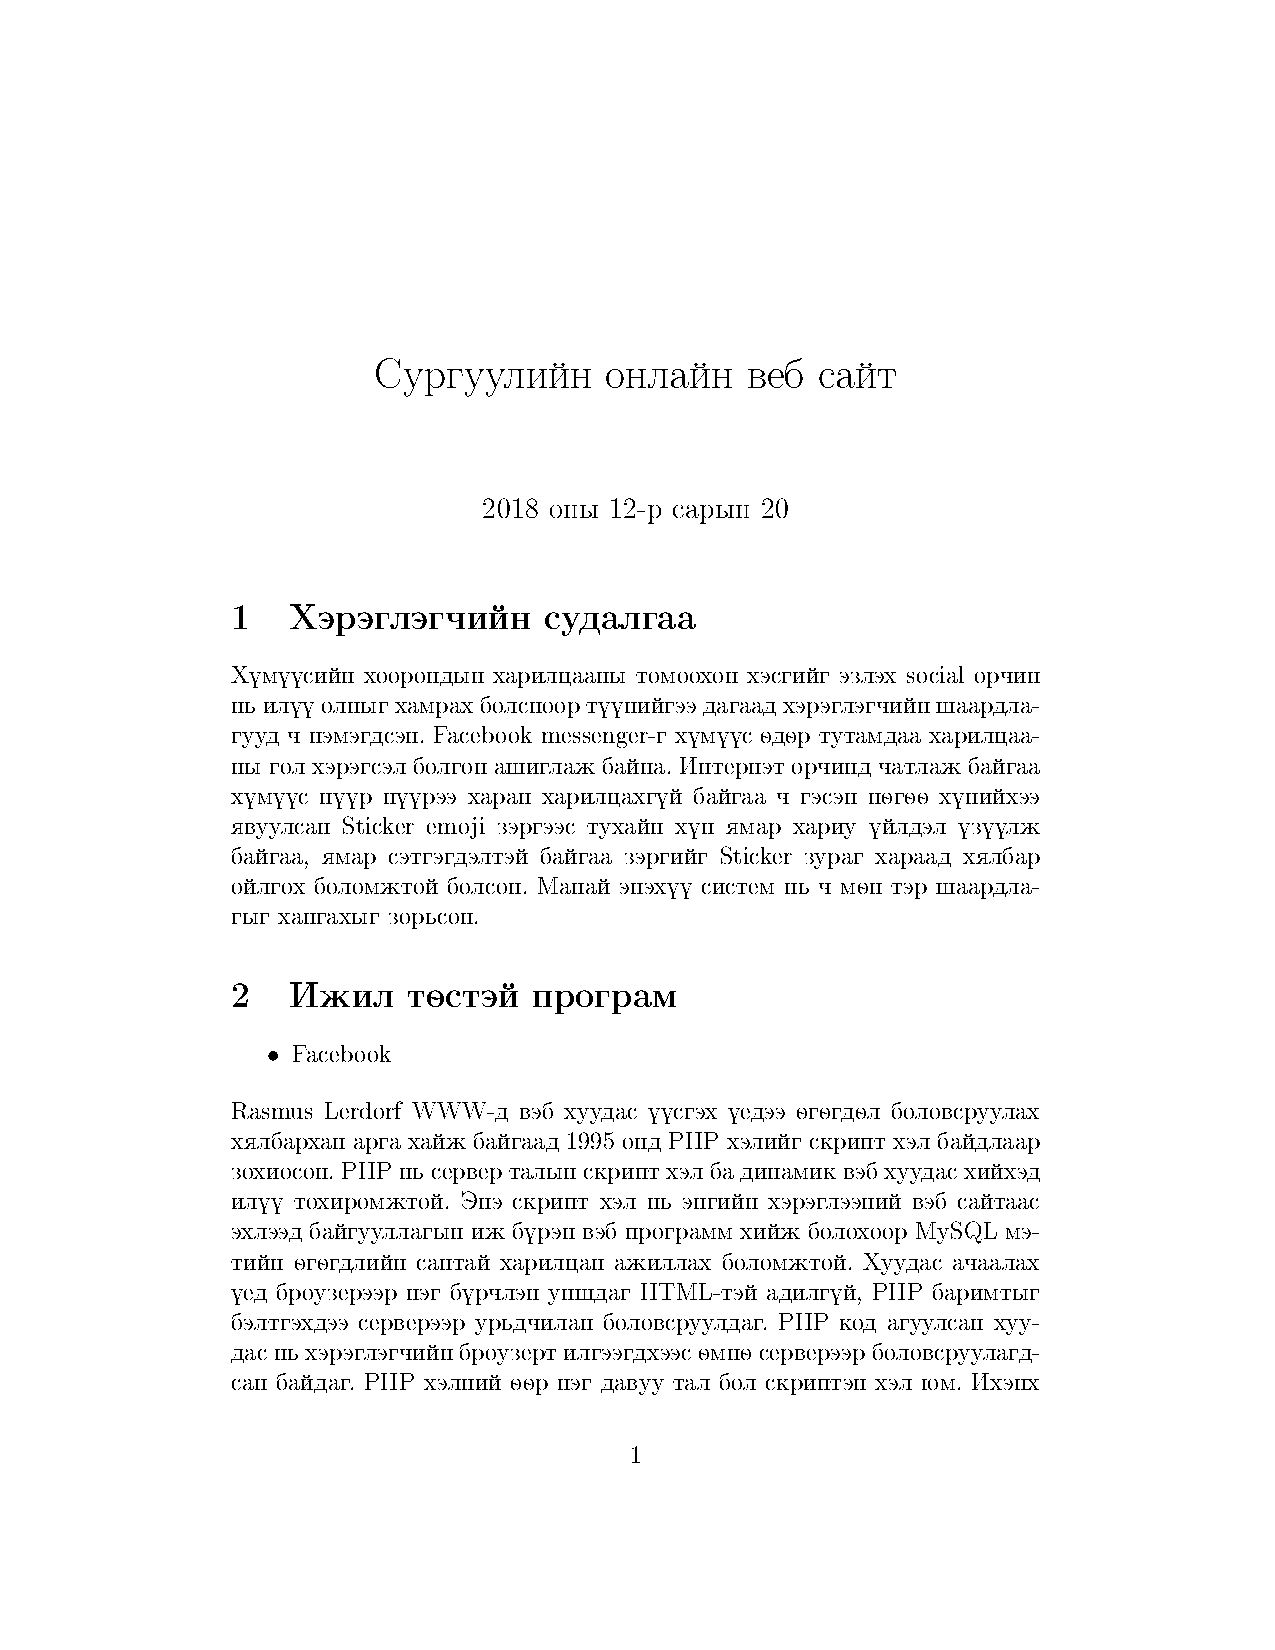
\includegraphics[width=\linewidth]{Sticker.jpg}
			\caption{BPMN.}
			\label{fig:bpmn1}
		\end{figure}
		\begin{figure}
		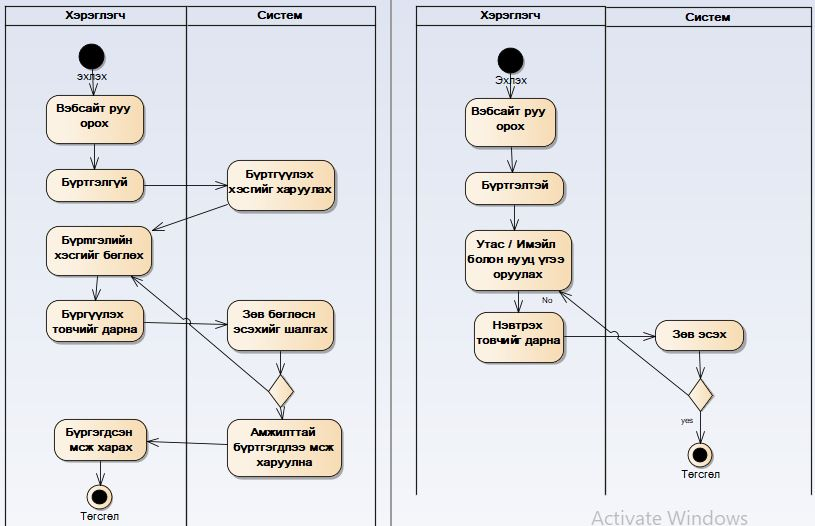
\includegraphics[width=\linewidth]{activity.jpg}
		\caption{Activity1.}
		\label{fig:activity1}
		\end{figure}
		\begin{figure}
		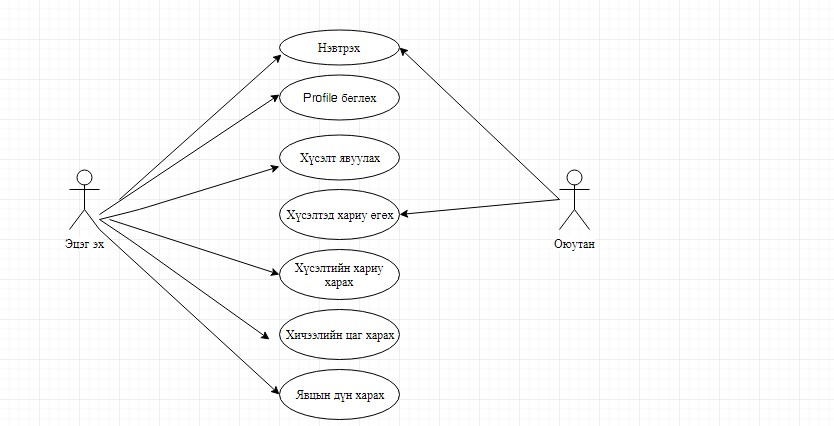
\includegraphics[width=\linewidth]{usecase.jpg}
		\caption{usecase.}
		\label{fig:usecase}
		\end{figure}
		\begin{figure}
		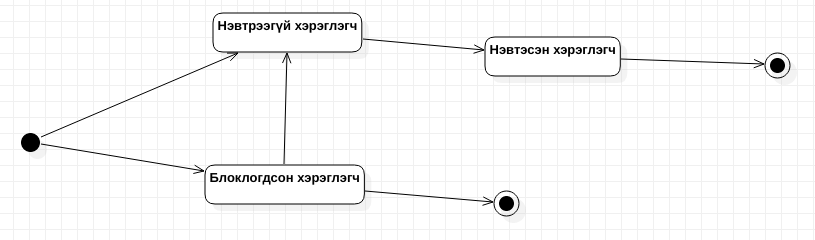
\includegraphics[width=\linewidth]{state.jpg}
		\caption{state.}
		\label{fig:usecase}
	\end{figure}
		\begin{figure}
		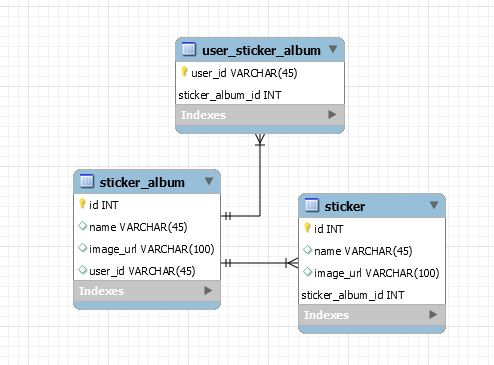
\includegraphics[width=\linewidth]{erd.jpg}
		\caption{erd.}
		\label{fig:erd}
	\end{figure}
	\begin{figure}
	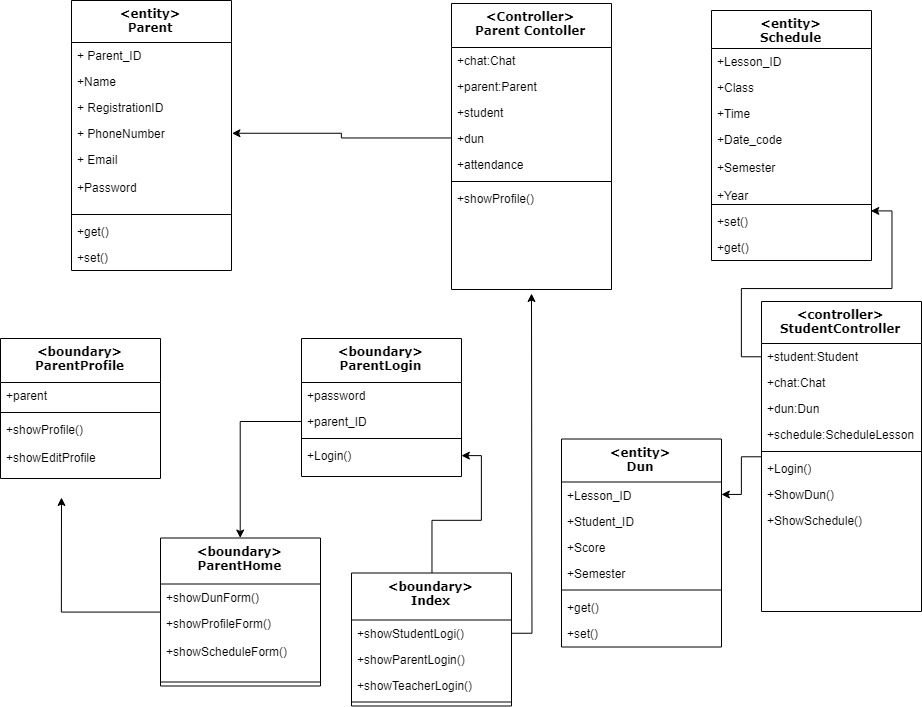
\includegraphics[width=\linewidth]{class.jpg}
	\caption{class.}
	\label{fig:erd}
\end{figure}
		\begin{figure}
		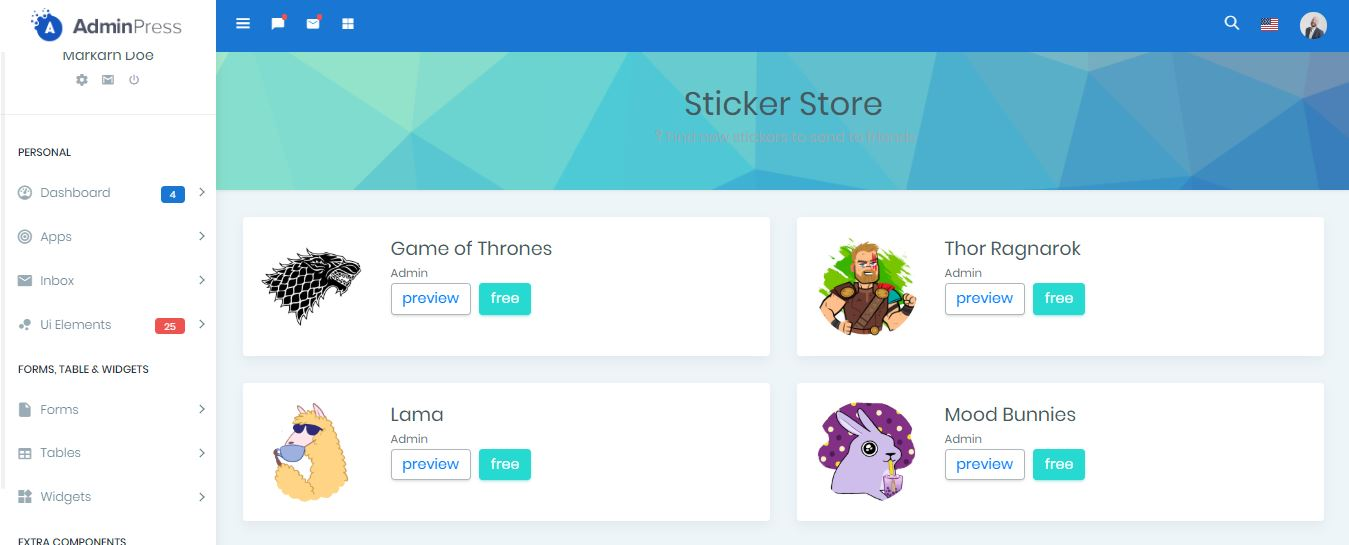
\includegraphics[width=\linewidth]{gui1.jpg}
		\caption{user gui.}
		\label{fig:erd}
	\end{figure}
	\begin{figure}
	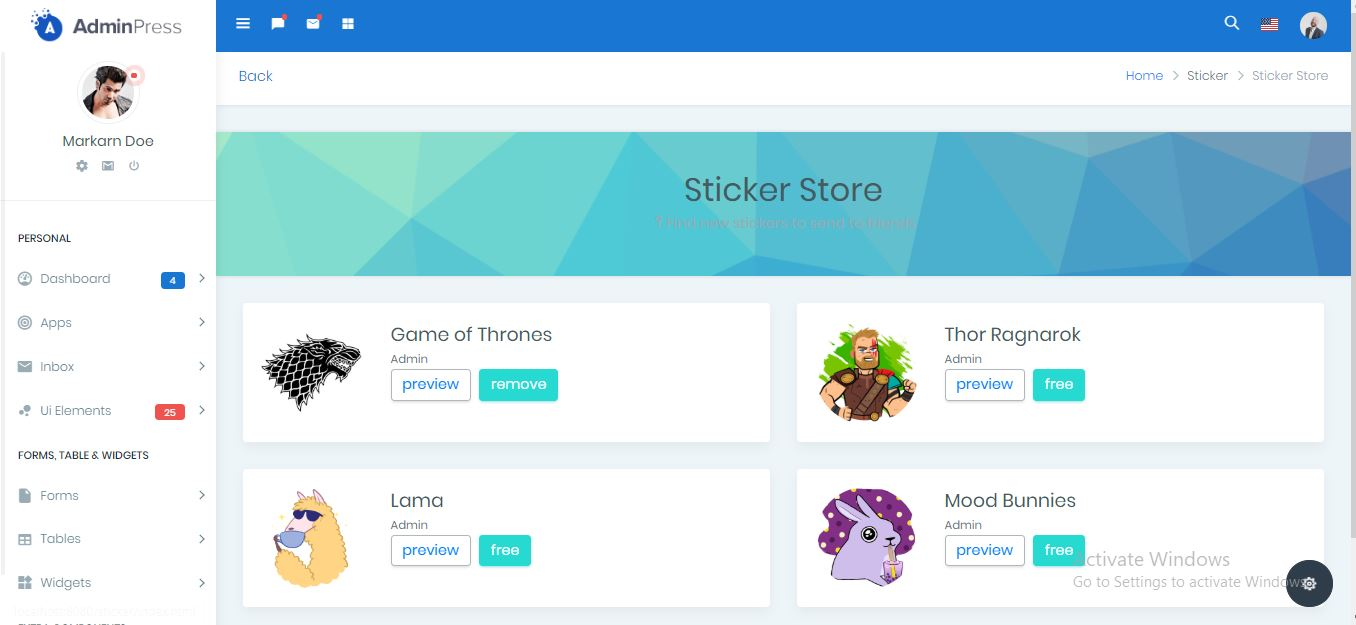
\includegraphics[width=\linewidth]{usergui.jpg}
	\caption{user gui.}
	\label{fig:erd}
\end{figure}
	\begin{figure}
	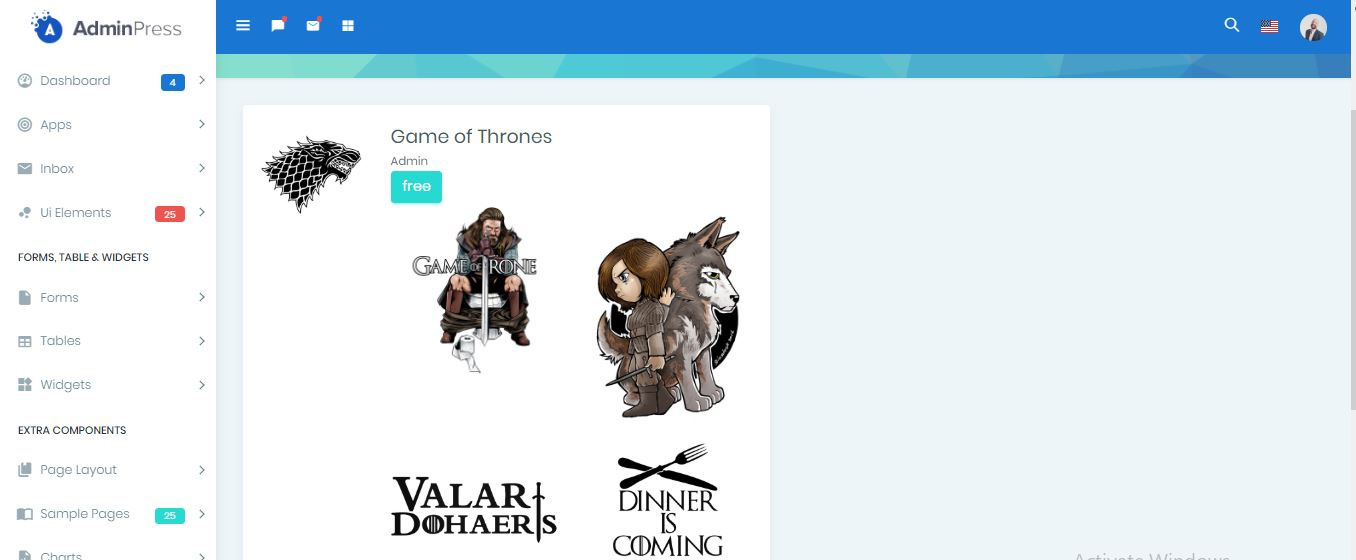
\includegraphics[width=\linewidth]{gui2.jpg}
	\caption{user gui.}
	\label{fig:erd}
	\end{figure}
	\begin{figure}
	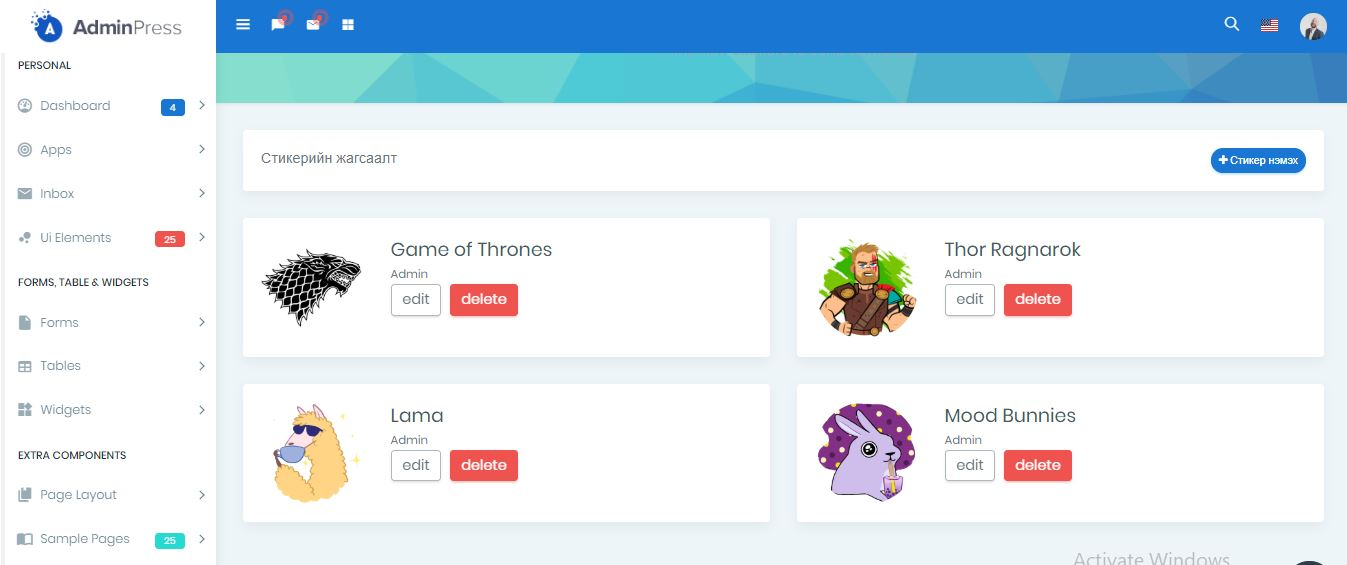
\includegraphics[width=\linewidth]{admin.jpg}
	\caption{admin gui.}
	\label{fig:erd}
\end{figure}
	\begin{figure}
	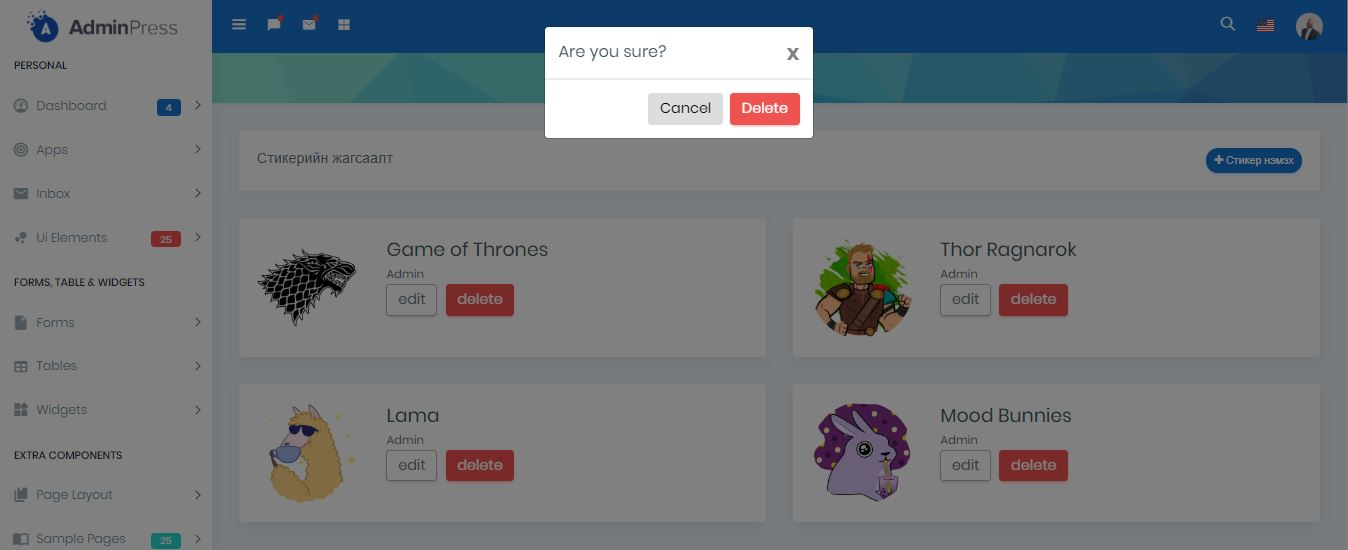
\includegraphics[width=\linewidth]{admindelete.jpg}
\caption{gui2.}
\label{fig:erd}
\end{figure}
	\begin{figure}
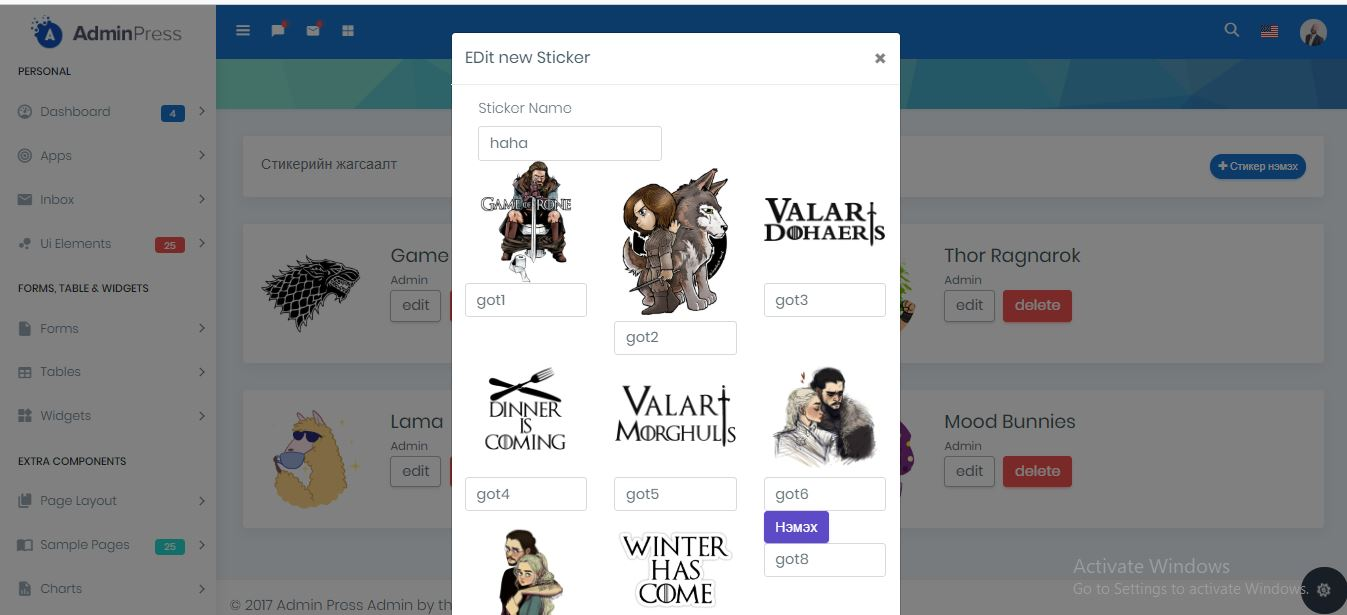
\includegraphics[width=\linewidth]{adminedit.jpg}
\caption{gui2.}
\label{fig:erd}
\end{figure}
	\begin{figure}
	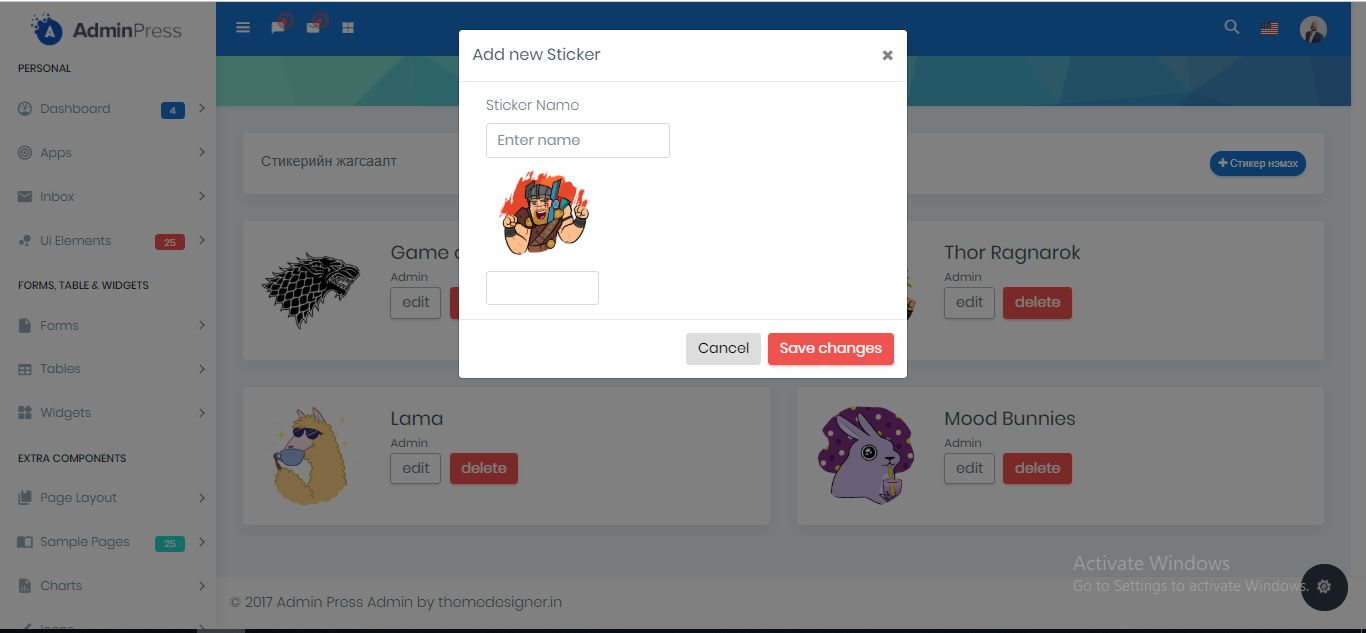
\includegraphics[width=\linewidth]{adminadd.jpg}
	\caption{gui2.}
	\label{fig:erd}
\end{figure}
\end{document}

